\vspace{-6mm}
\section{}
Experiment 1 에서는 MAC (Medium Access Control Layer) 의 contention - based protocol 인 ALOHA의 동작에 대해서 simulation을 진행한다. 
pre report 에서 pure aloha 와 slotted aloha 의 각각 포아송 분포를 가정하는 전송량 G -load 에 따른  이론적인 Throughput의 graph가 각각 $G\times e^{-G},\ G\times e^{-2G}$   를 확인한것과 같이, omnetpp simulatino 을 통해서 pure aloha 와 slotted aloha 각각의   G-load 가 일반의 경우와  optimal인 경우 4가지에 대한  simulation을 진행한다.
\vspace{-2mm}
\subsection{}
    \vspace{-2mm}
    \subsubsection{ini simulation file setting}
    \vspace{-2mm}
    4개의 simulation setting code는 다음과 같다. 각각의 G-load 를 iaTime variable을 통해서 설정한것을 확인할 수 있다.
            \vspace{-2mm}
            \begin{listing}[h!]
            \inputminted[framerule = 1pt,framesep = 2mm , frame = lines, fontsize=\scriptsize ]{c}{./code/week12/Experiment_01/ini.cpp}
            \vspace{-3mm}
            \caption{\footnotesize aloha ini file}
            \end{listing}
            \vspace{-6mm}
    \subsubsection{Simulation Results : Sequence Chart}
    \vspace{-3mm}
    Aloha의 실험결과로 각 simulatino Time 기준으로 10초를 진행하여 생성한 event log를 바탕으로 sequence log와 scalar file 로부터 channel util($\sim$ Throughput) 값을 얻을 수 있었다.
    
    결과 차트는 아래와 같다. 1번쨰 2번째는 Pure Aloha의 G-load 1/6 과 optimal 인 1/2 의 결과로 총 3 sec 가 표기되도록 sequence log 차트의screenshot을 캡처했다. G-load가 3배가 더 만큼 동일시간 동안 3배 더많은 전송이 진행된 것과 pure aloha의 특성상 전송시간이 fix 되지않아 많은 collision이 발생한것을 확인할 수 있다.
    
    3번째, 4번째 Slotted Alohs의 G-load가 1/4 와 optimal 인 1 의 결과로 총 2 sec가 표기되도록 sequence log 차트의screenshot을 캡처했다. 마찬가지로 G-load가 4배 정도 차이가 있지만 slot동안 전송이 요청되는 frame 에 대해서 slot과 slot 사이에서만 전송되는 slotted aloha 의 workflow를 확인할 수 있었고, 각각 pure aloha 보다 collision이 현격히 감소한 것을 확인할 수 있었다. 구체적인 수치는 scalar file에서 확인한 채널효율로 비교해보고자 한다. 
    \clearpage
        \begin{figure}[h!]
        \centering
        \subfloat[Aloha, frequent transmission (high collision rate)]{
            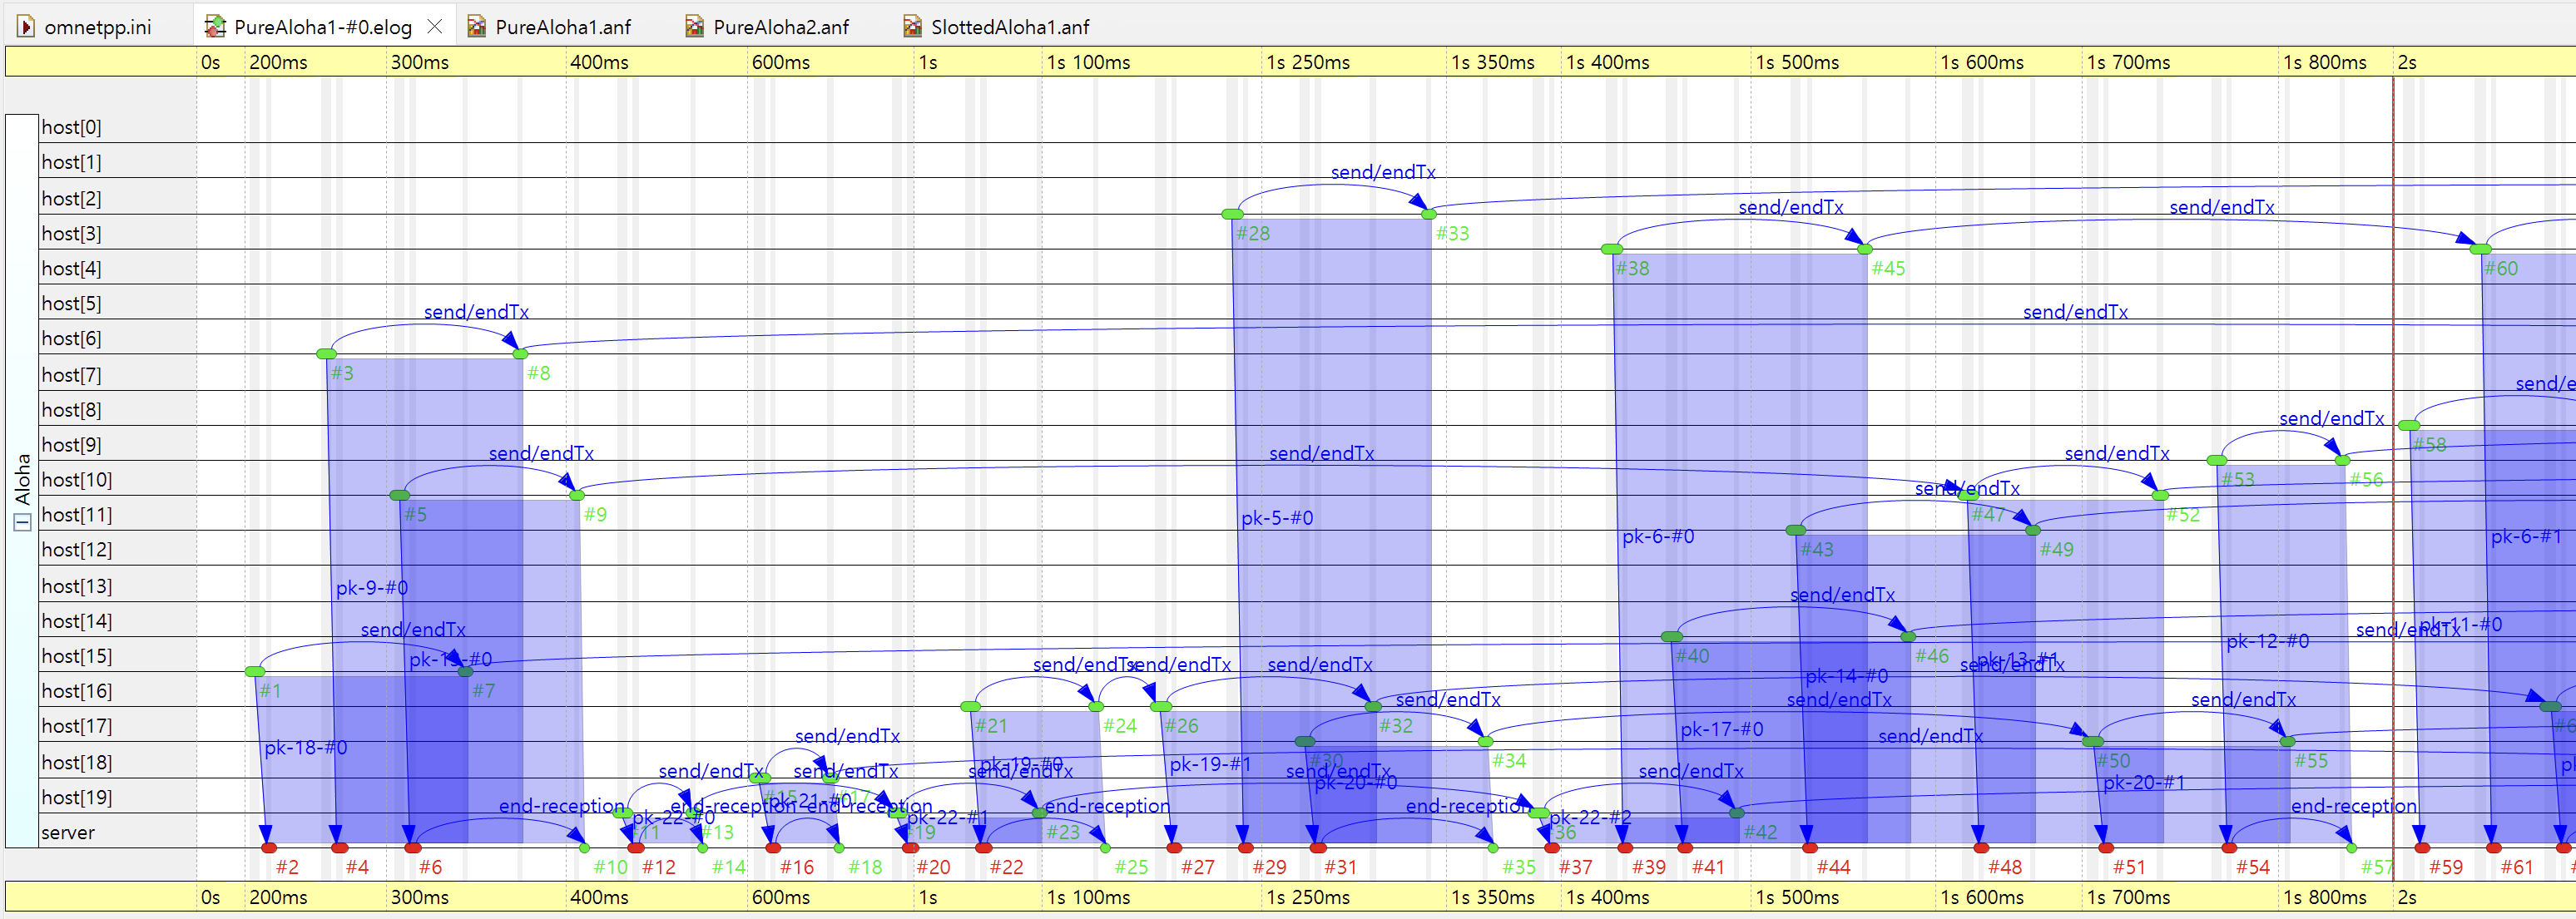
\includegraphics[width=0.93\textwidth]{image/week12/1-1-1.png}
        }\hspace{3mm}
        \subfloat[Aloha, optimal load]{
            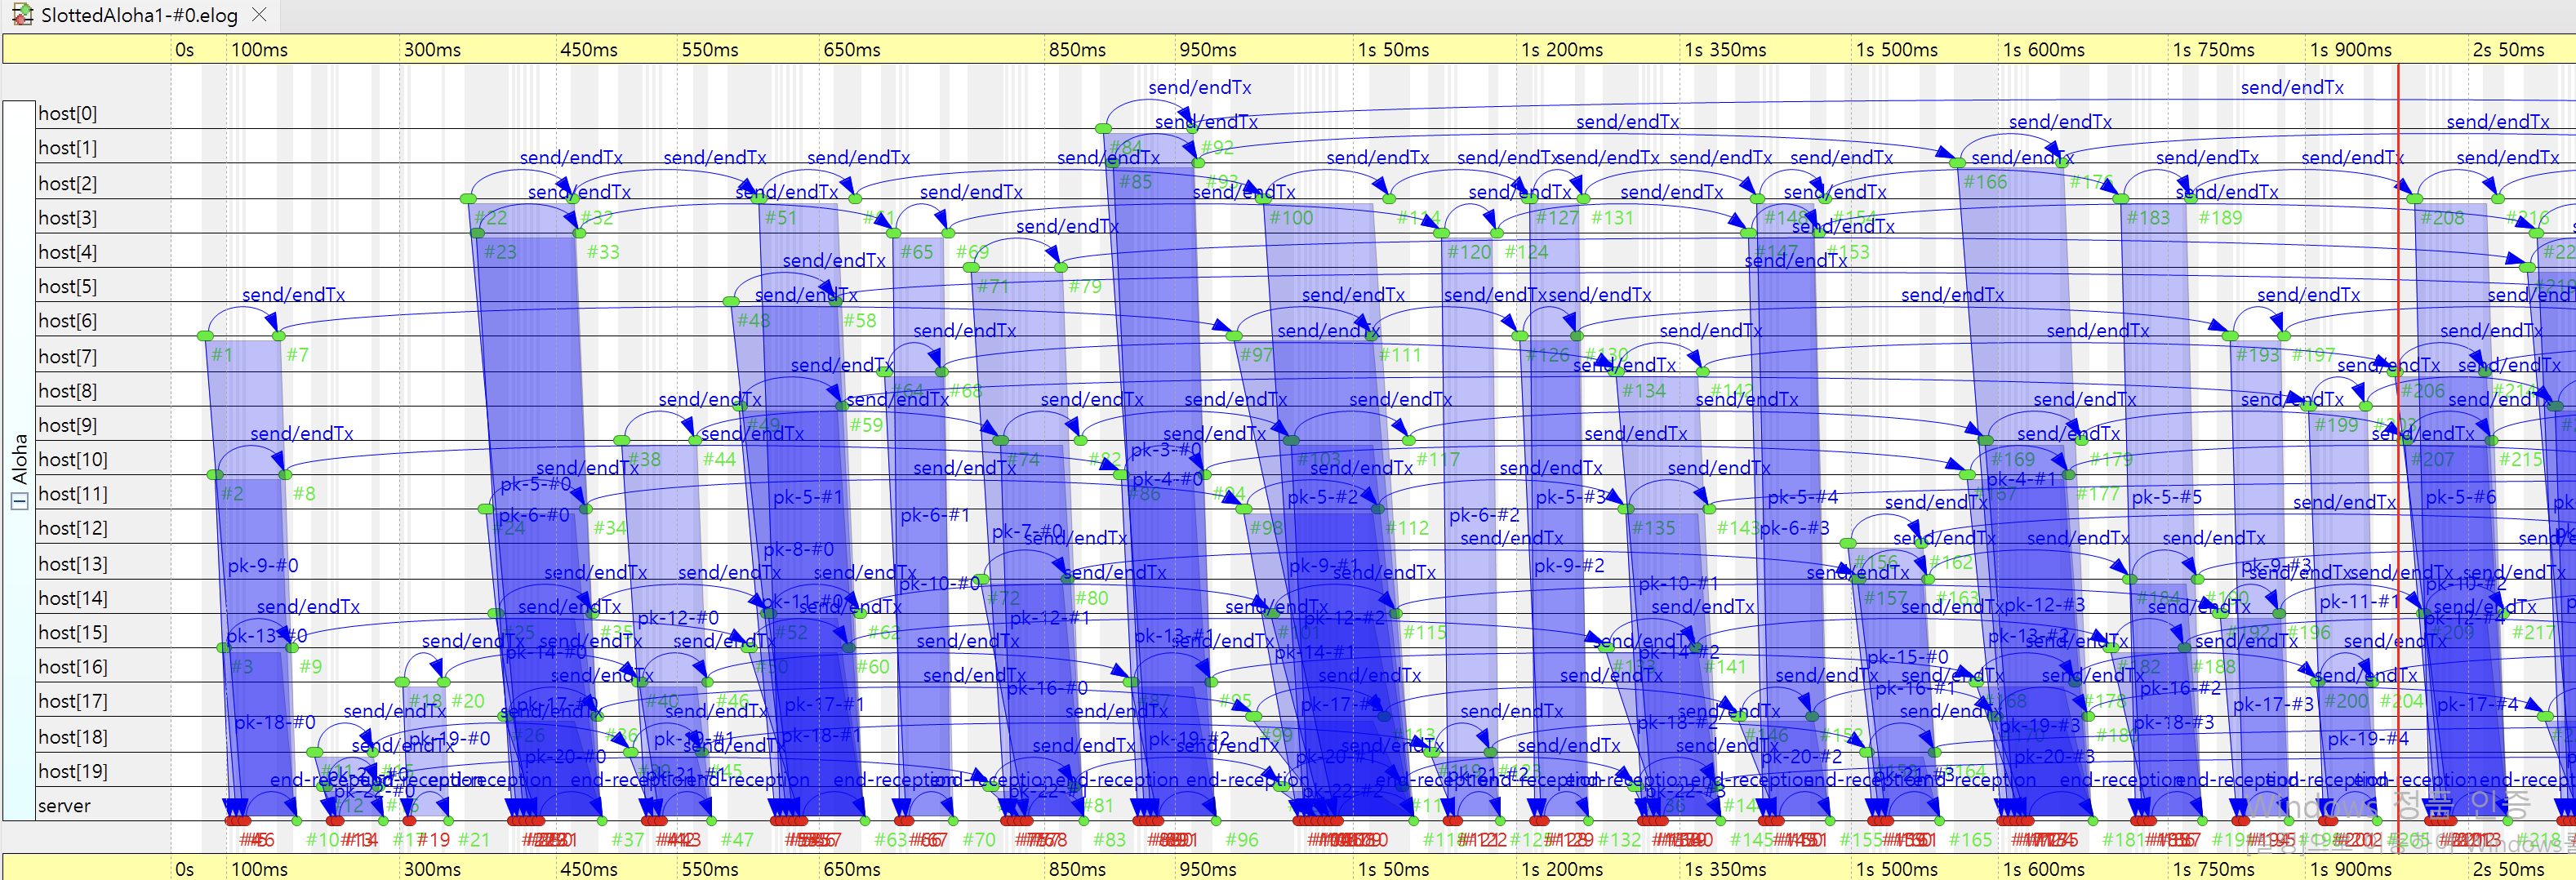
\includegraphics[width=0.93\textwidth]{image/week12/1-1-2.png}
        }\hspace{3mm}
        \subfloat[Slotted Aloha, frequent transmission (high collision rate)]{
            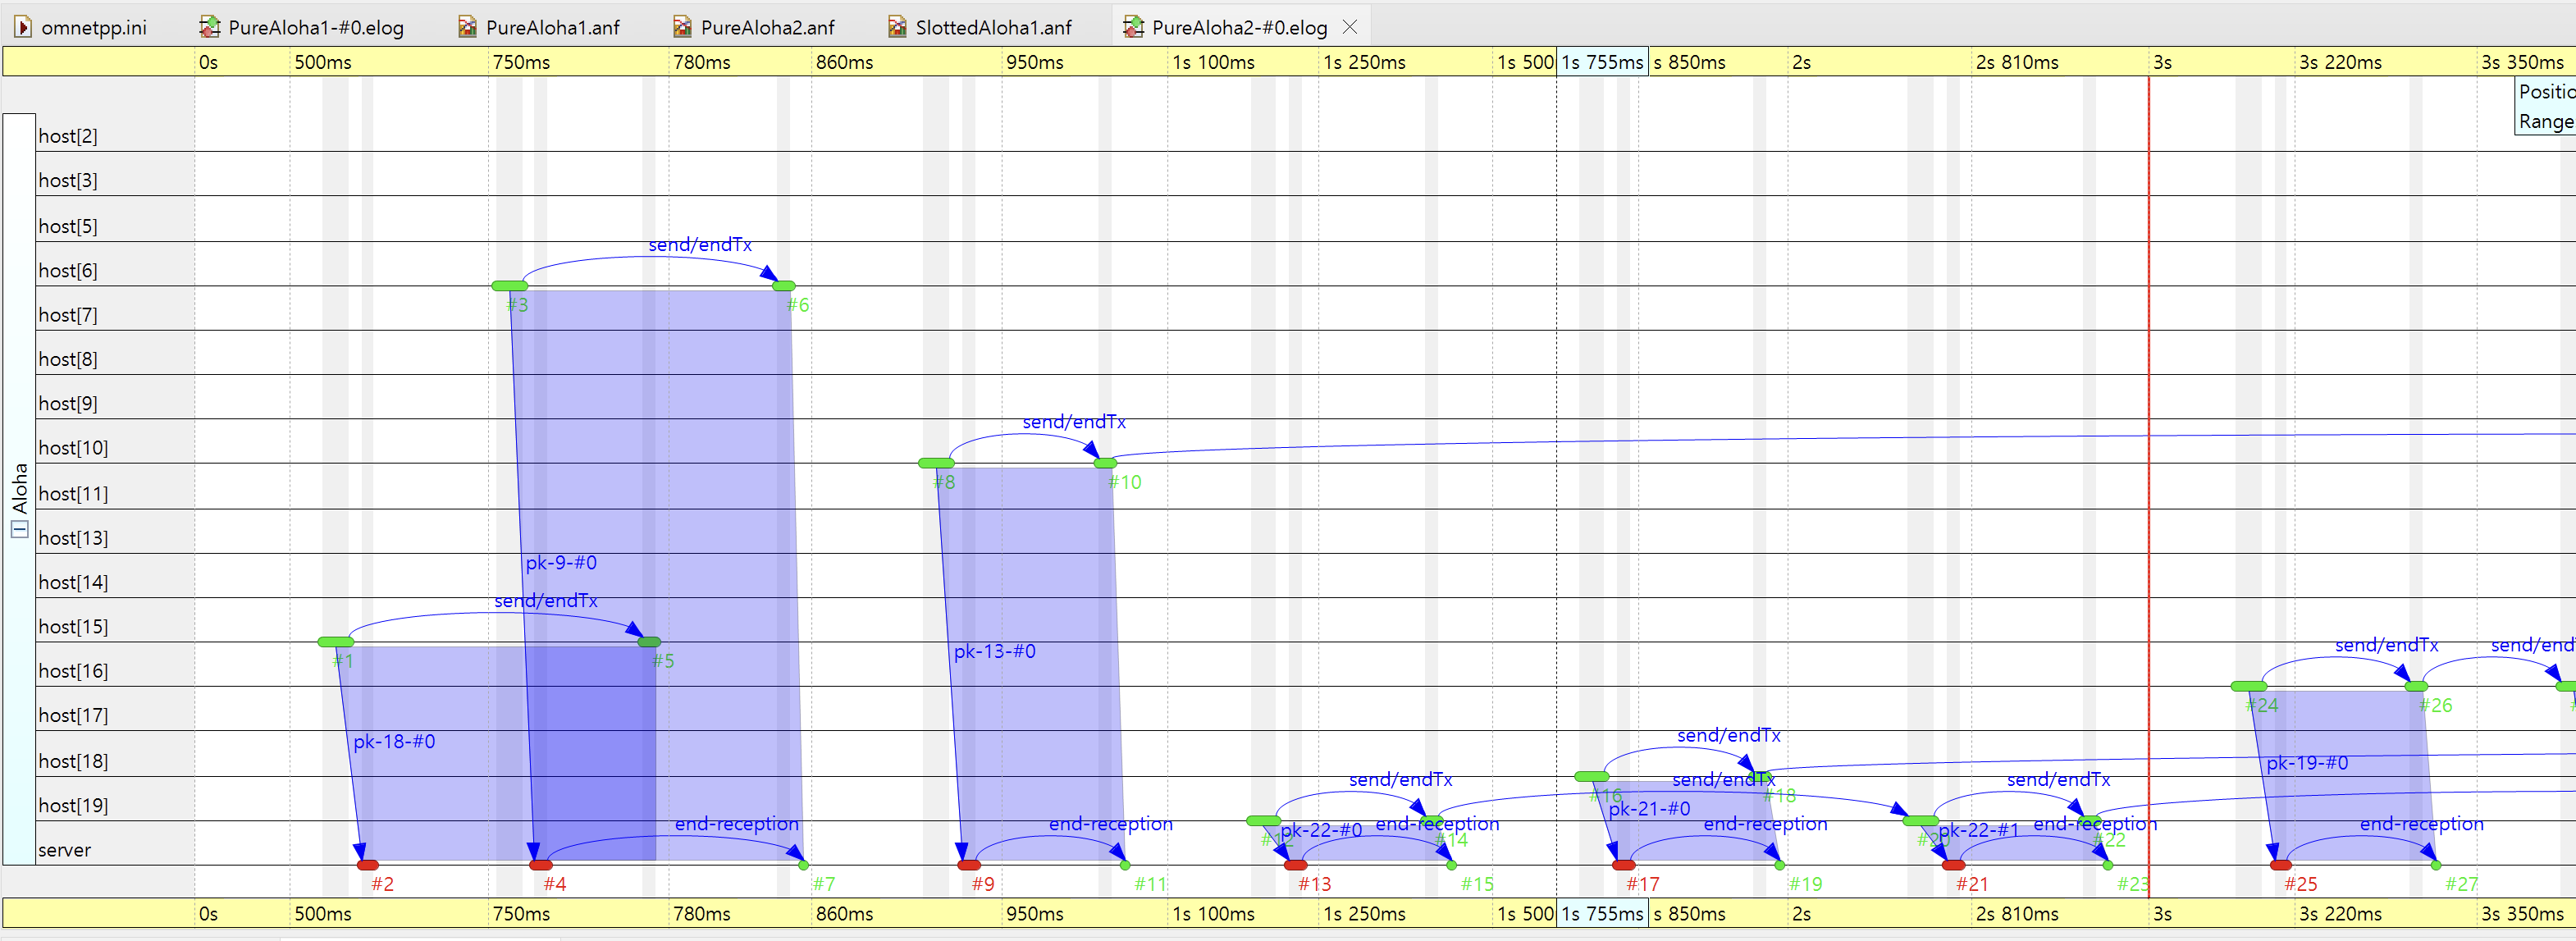
\includegraphics[width=0.93\textwidth]{image/week12/1-1-3.png}
        }\hspace{3mm}
        \subfloat[Slotted Aloha, optimal load]{
            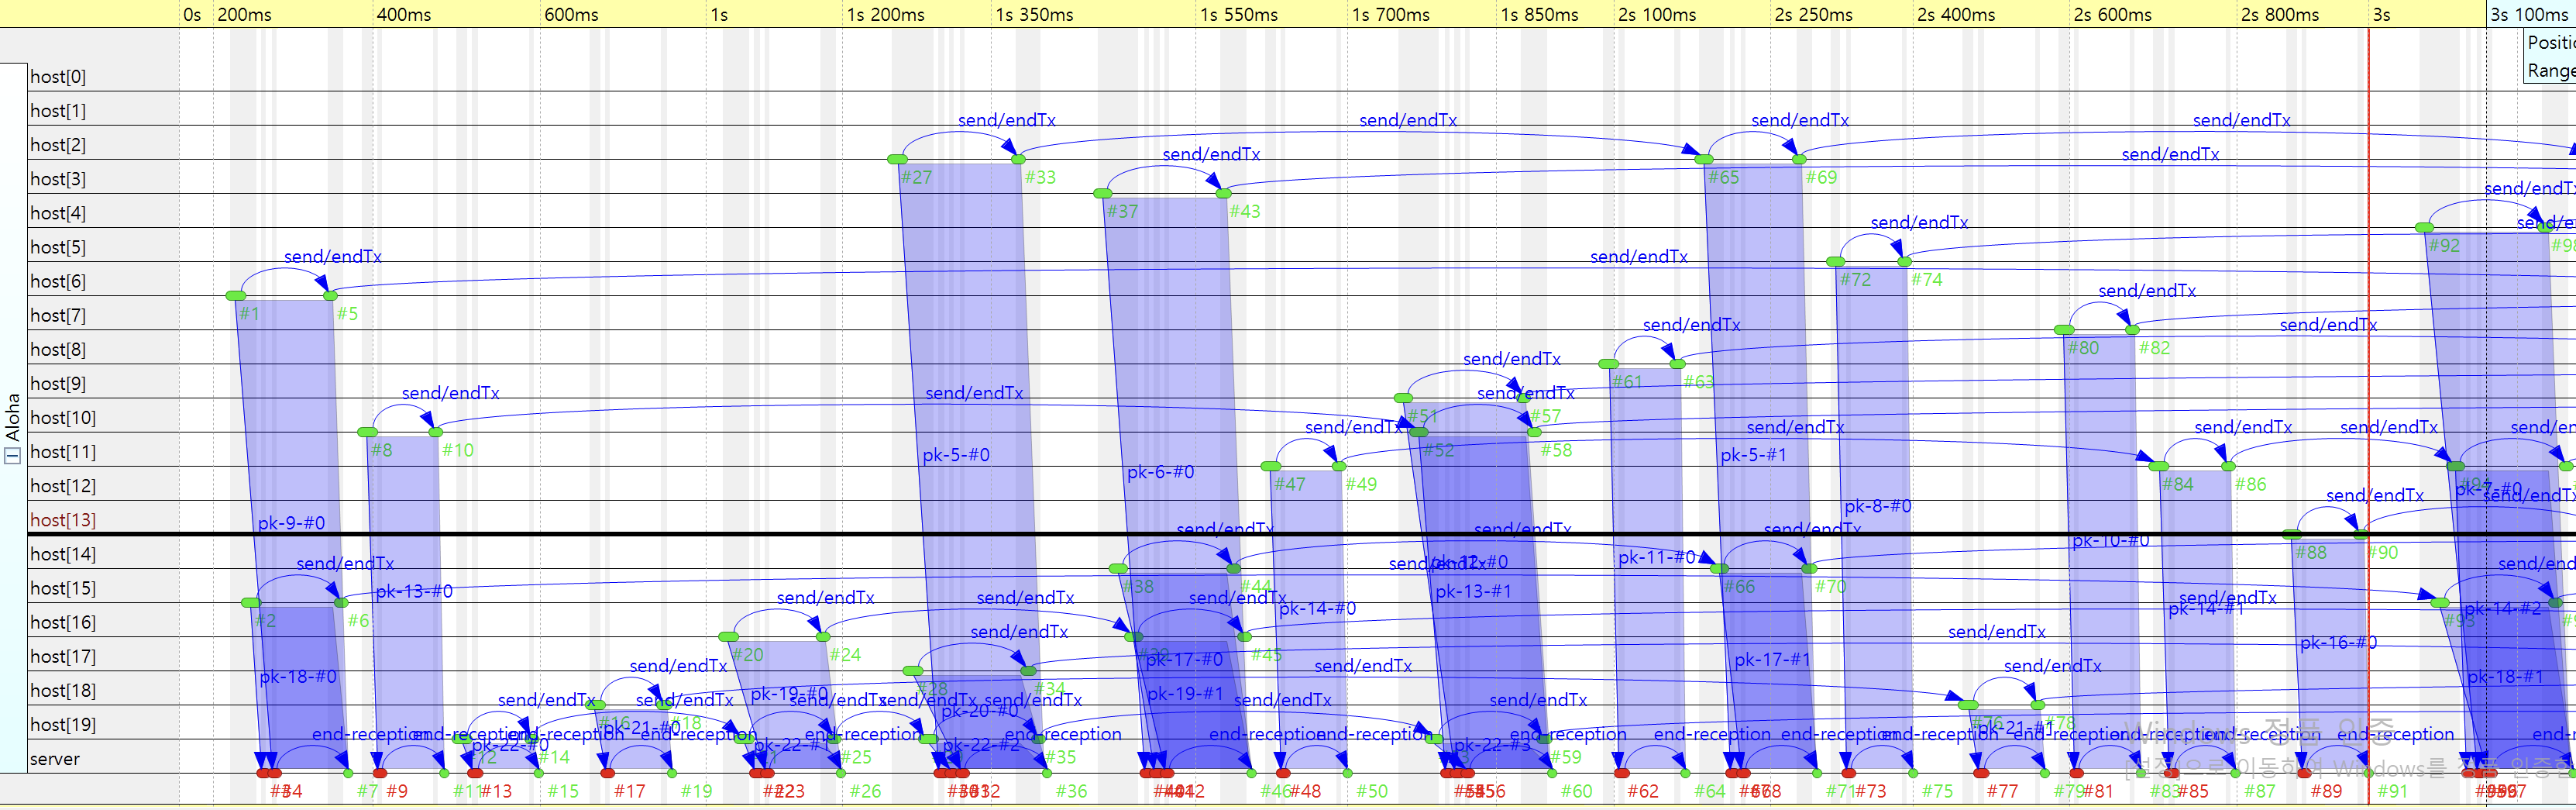
\includegraphics[width=0.93\textwidth]{image/week12/1-1-4.png}
        }
        \vspace{-2mm}
        \caption{Experiment 1-1 Simulation Results Screenshot: Aloha simulation sequence log}
        \end{figure}
     \clearpage